\subsection{Nyquist-Plot}

Die Ortskurve oder auch Nyquist-Plot in Abbildung \ref{fig:nyquist-plot} ist ein Graph, der die Amplitude und Phase des Systems für Schwingungen mit allen Frequenzen darstellt.

\begin{figure}[H]
	\centering
	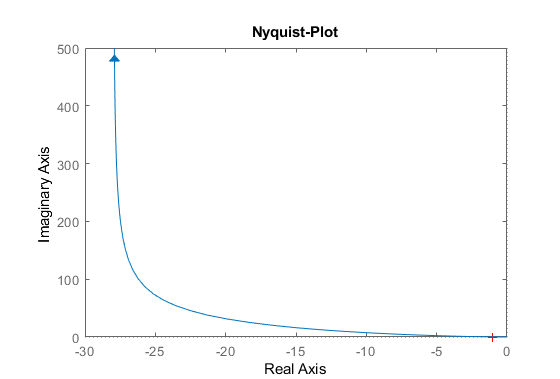
\includegraphics[width=0.7\linewidth]{diagrams/nyquistDiagram.png}
	\caption[Nyquist-Plot]{Nyquist-Plot}
	\label{fig:nyquist-plot}
\end{figure}